\documentclass[12pt,spanish]{article}
\usepackage[spanish]{babel}
\usepackage{graphicx}
\usepackage{color}
\usepackage{xcolor}
\usepackage{colortbl}
\usepackage{amsthm,thmtools}
\usepackage{multirow}
\usepackage{amsmath}
\usepackage{subcaption}
\usepackage{adjustbox}
\usepackage{multirow}
\usepackage[hidelinks]{hyperref}
\usepackage{caption}
\usepackage{amsthm}
\usepackage{multicol}
\usepackage{float}
\usepackage{amsfonts}
\usepackage{titling}
\usepackage{soul}
\usepackage{listings}
\usepackage{array}
\usepackage{tikz}
\usetikzlibrary{shapes.geometric, arrows, chains, calc,positioning,fit,decorations.pathreplacing}
\usepackage[framemethod=tikz]{mdframed}

\graphicspath{ {../img/}}
\selectlanguage{spanish}
\usepackage[utf8]{inputenc}
\usepackage{graphicx}
\usepackage[a4paper,left=3cm,right=2cm,top=2.5cm,bottom=2.5cm]{geometry}

\newenvironment{solution}{
	\par
	\textbf{Solución}
	\par
	\begin{center}
}
{
	\end{center}
}


\title{Ingeniería de Servidores}
\setlength{\droptitle}{10em}
\author{Carlos Sánchez Páez}

\makeindex
\begin{document}
\definecolor{light-gray}{gray}{0.95}
\lstset{columns=fullflexible,basicstyle=\ttfamily}
\surroundwithmdframed[
  hidealllines=true,
  backgroundcolor=light-gray,
  innerleftmargin=0pt,
  innertopmargin=0pt,
  innerbottommargin=0pt]{lstlisting}


\begin{titlepage}

 \newlength{\centeroffset}
 \setlength{\centeroffset}{-0.5\oddsidemargin}
 \addtolength{\centeroffset}{0.5\evensidemargin}
 \thispagestyle{empty}

 \noindent\hspace*{\centeroffset}
 \begin{minipage}{\textwidth}

  \centering
  
\includegraphics[width=0.9\textwidth]{logo_ugr.jpg}\\[1.4cm]

  \textsc{ \Large Ingeniería de Servidores\\[0.2cm]}
  \textsc{GRADO EN INGENIERÍA INFORMÁTICA}\\[1cm]

  {\Huge\bfseries Guión de prácticas resueltas\\}
 \end{minipage}

 \vspace{1.5cm}
 \noindent\hspace*{\centeroffset}
 \begin{minipage}{\textwidth}
  \centering

  \textbf{Autor}\\ {Carlos Sánchez Páez}\\[2.5ex]
  
\includegraphics[width=0.4\textwidth]{etsiit_logo.png}\\[0.1cm]
  \vspace{1.5cm}
  
\includegraphics[width=0.15\textwidth]{atc.jpg}\\[0.1cm]
  \vspace{1cm}
  \textsc{Escuela Técnica Superior de Ingenierías Informática y de Telecomunicación}\\
  \vspace{1cm}
  \textsc{Curso 2019-2020}
 \end{minipage}
\end{titlepage}
\thispagestyle{empty}
\newpage
\tableofcontents{}
\newpage
\listoffigures
\thispagestyle{empty}
\newpage

\section{Práctica 1: Virtualización e instalación de Sistemas Operativos}

\subsection{Sesión 1}

\subsubsection{Tipos de arquitecturas}

Un servidor es una máquina que se dedica a resolver peticiones. Hay varios tipos:
\begin{itemize}
  \item \textbf{Hosting dedicado}. Alguien monta su propio servidor y únicamente lo utiliza él.
  \item \textbf{VPS (\textit{Virtual Private Server})}. Se utiliza la virtualización para proporcionar recursos dedicados (privados) al cliente a partir de un servidor con múltiples usuarios.
  \item \textbf{\textit{Serverless}}. Se necesita un proveedor cloud (\textit{AWS, Azure, Google Cloud}...), que gestiona dinámicamente los recursos. Las aplicaciones se ejecutan al detectarse determinados eventos. Se cobra por ancho de banda utilizado, capacidad de disco duro, etc. La principal ventaja de esta arquitectura es la escalabilidad.
\end{itemize}

\begin{figure}[H]
  \centering
  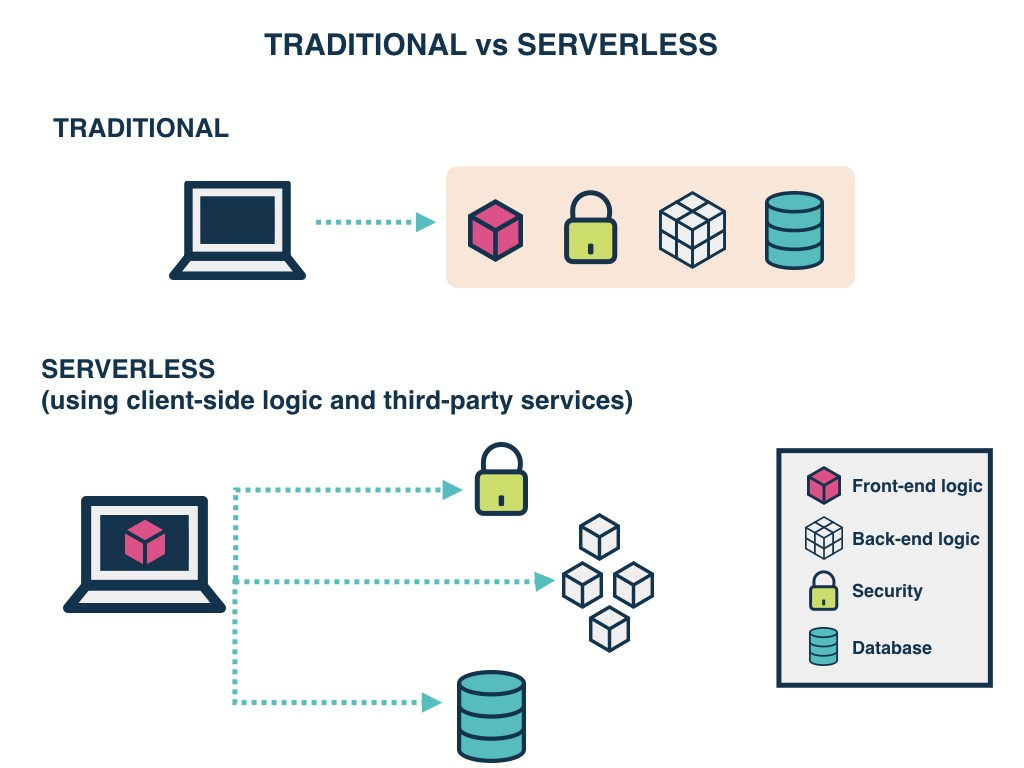
\includegraphics[width=0.55\textwidth]{serverless.jpeg}
  \vspace{0.5cm}
  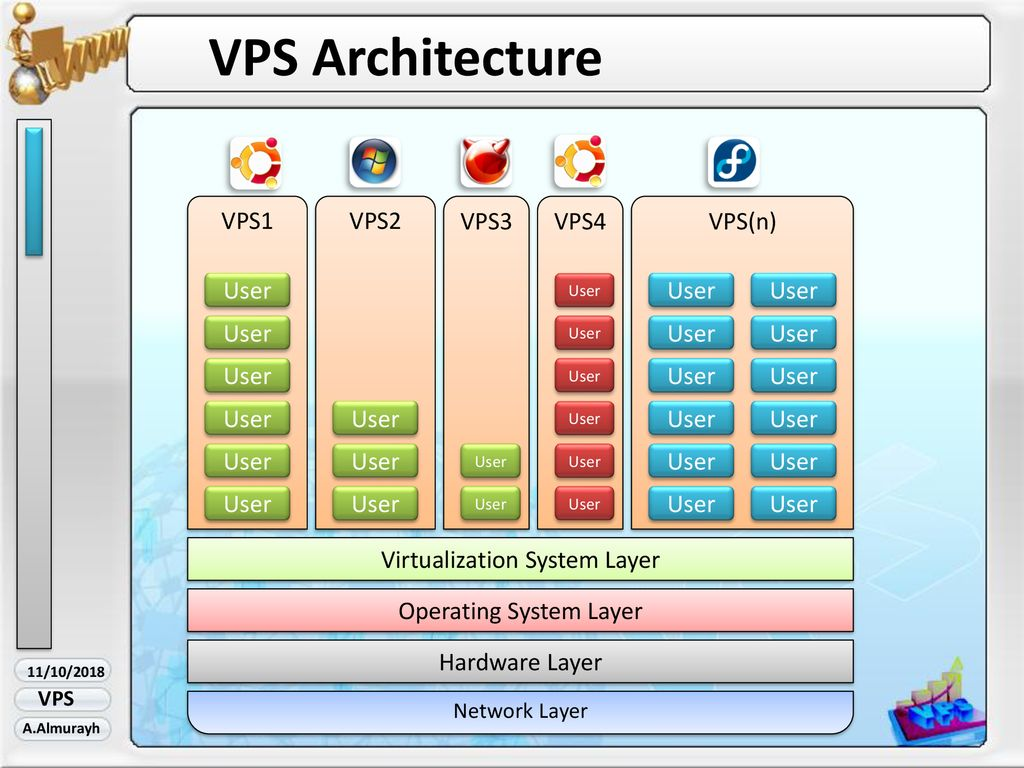
\includegraphics[width=0.55\textwidth]{vps.jpg}
  \caption{Tipos de arquitecturas de servidor}
\end{figure}

Una \textbf{máquina virtual} es aquella en la que todo su \textit{hardware} está virtualizado, es decir, compartido con el host. Las principales ventajas de las MV son precio, encapsulamiento y flexibilidad. Realmente no son más que archivos.\\

Un \textbf{contenedor} empaqueta una aplicación con sus correspondientes dependencias, consiguiendo así la máxima \textit{portabilidad}. Lo único que se necesita tener instalado en una máquina para ejecutar la aplicación es necesario contar con el hipervisor adecuado (por ejemplo, \textit{Docker}).\\

Un \textbf{hipervisor} es un motor que se encarga de traducir las instrucciones de una máquina virtual (o contenedor) a llamadas al sistema. Algunos ejemplos de hipervisor son \textit{VirtualBox} o \textit{VMWare}.

\begin{figure}[H]
  \centering
  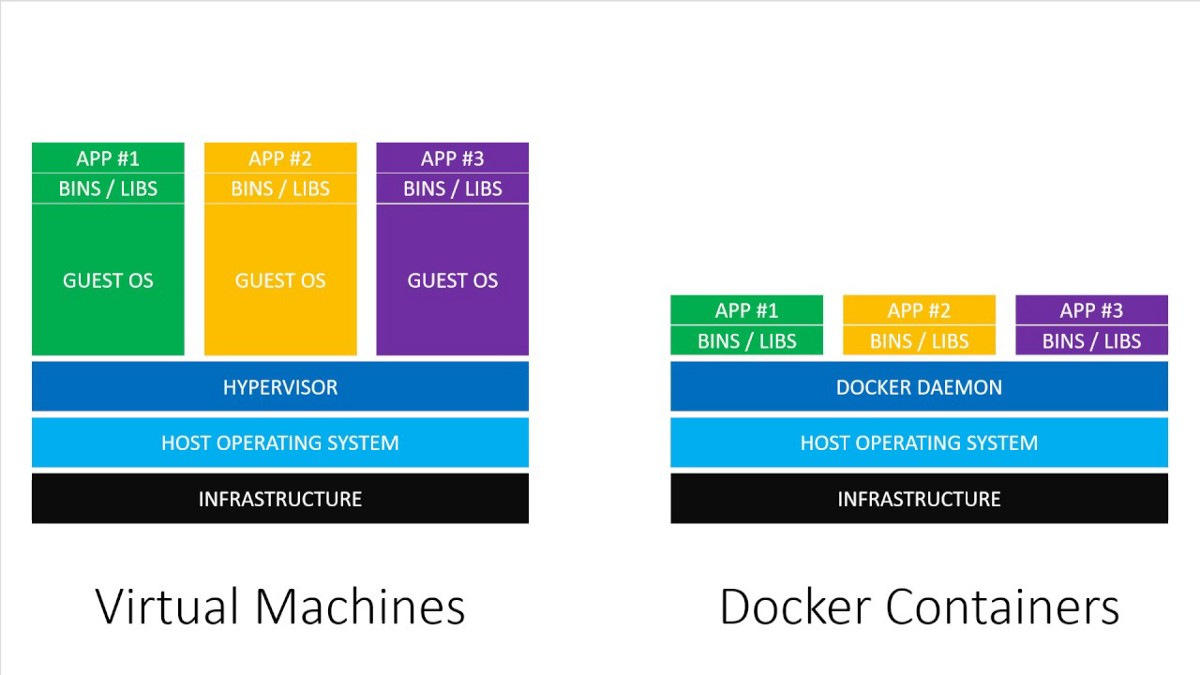
\includegraphics[width=\textwidth]{contenedor_vs_vm.jpeg}
  \caption{Diferencias entre contenedor y máquina virtual}
\end{figure}
Podríamos realizar una analogía diciendo que las máquinas virtuales son procesos (encapsulados, no pueden acceder entre ellos) y los contenedores son hebras (sí que pueden comunicarse).

\subsubsection{RAID}

RAID (\textit{\textbf{R}edundant \textbf{A}rray of \textbf{I}ndependent/\textbf{I}nexpensive} \textbf{D}isks) es una tecnología que utiliza varias unidades de almacenamiento entre las que se replican los datos. Existen varios tipos de RAID:
\begin{itemize}
  \item \textbf{RAID0}. En este modelo no hay réplica. Los datos se distribuyen equitativamente entre ambos volúmenes.
  \item \textbf{RAID1}. Los datos se copian en el otro disco (espejo).
  \item \textbf{RAID2,3,4} no se usan en la actualidad.
  \item \textbf{RAID5}. Implementa bloques de paridad como medida de redundancia. Puede fallar un disco como máximo.
  \item \textbf{RAID6}. Implementa doble paridad. Pueden fallar dos discos como máximo.
  \item \textbf{RAID0+1,RAID1+0}. Se anidan ambos tipos de RAID.
\end{itemize}

\begin{figure}[H]
  \centering
  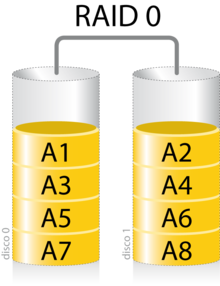
\includegraphics[width=0.2\textwidth]{raid0.png}
  \hspace{0.5cm}
  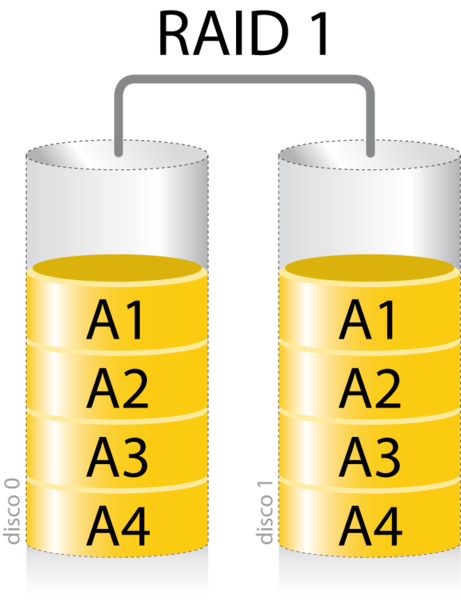
\includegraphics[width=0.2\textwidth]{raid1.png}
  \\
  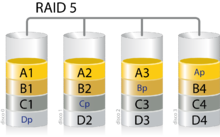
\includegraphics[width=0.4\textwidth]{raid5.png}
  \hspace{0.5cm}
  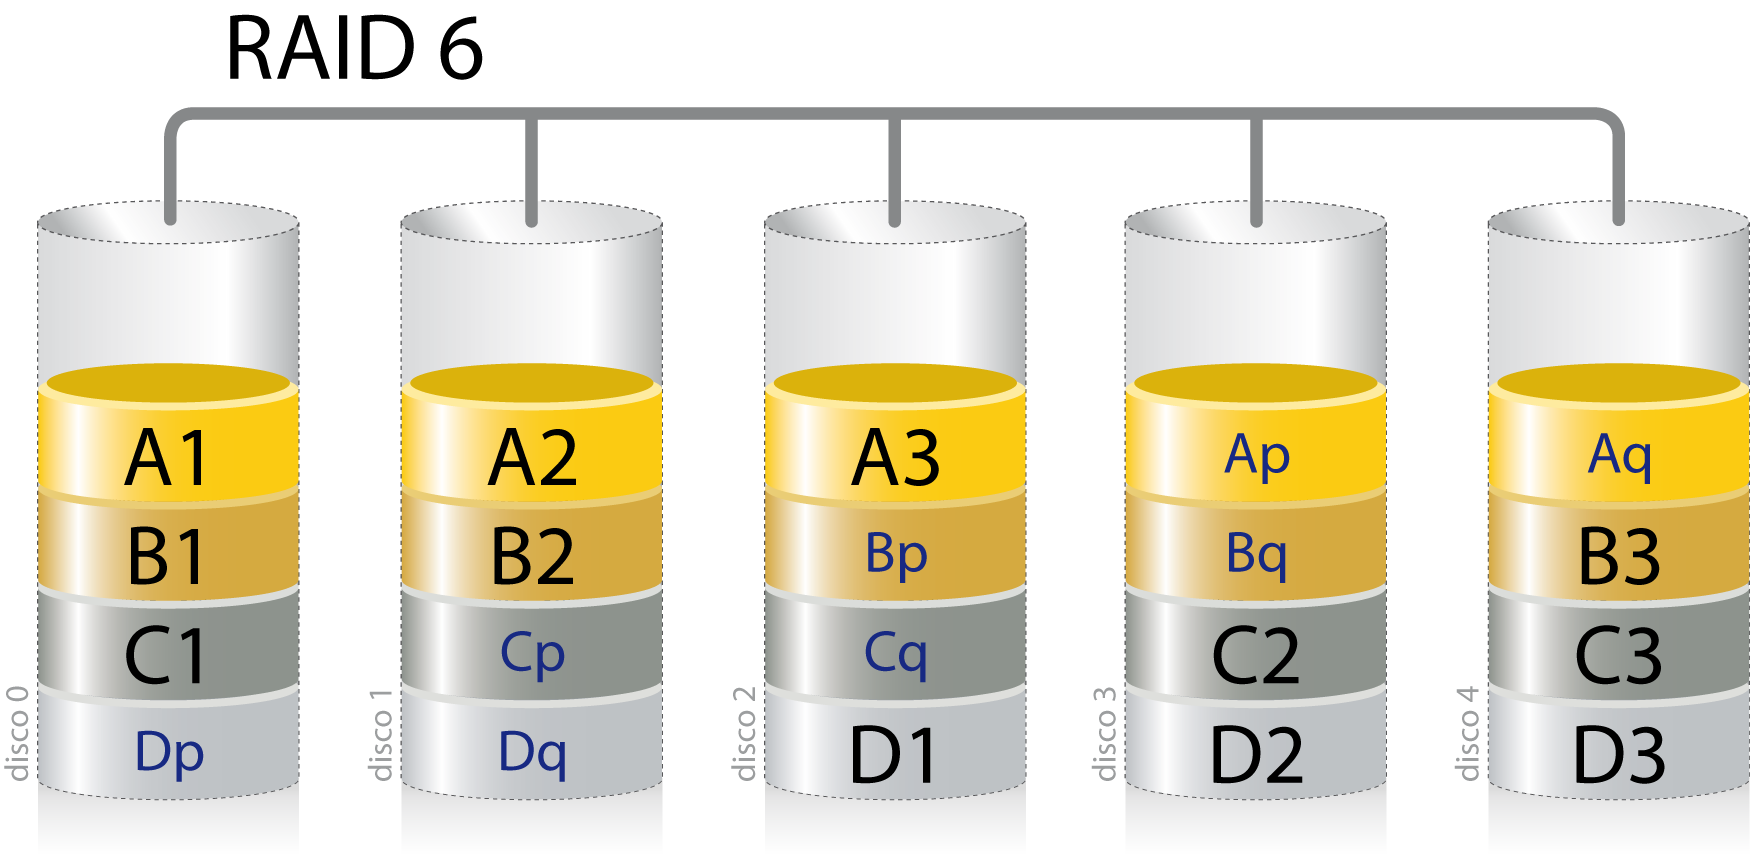
\includegraphics[width=0.4\textwidth]{raid6.png}
  \\
  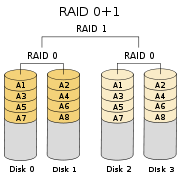
\includegraphics[width=0.4\textwidth]{raid01.png}
  \hspace{0.5cm}
  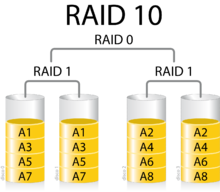
\includegraphics[width=0.4\textwidth]{raid10.png}
  \caption{Tipos de RAID}
\end{figure}

\newpage

\subsubsection{LVM}
LVM (\textit{\textbf{L}ogical \textbf{V}olume \textbf{M}anager}) provee abstracción sobre el almacenamiento físico y el sistema de ficheros. Sus mayor ventaja es la flexibilidad: podemos incorporar nuevas unidades de almacenamiento \textit{en caliente} (sin parar el sistema) de forma sencilla. LVM está compuesto por:
\begin{itemize}
  \item Volumen físico (\textit{Physical Volume}, \textbf{PV}). Es un dispositivo de almacenamiento (HDD, partición, RAID...).
  \item Grupo de volúmenes (\textit{Volume Group}, \textbf{VG}). Es el centro de LVM. Está formado por uno o más PV. Para aumentar su espacio sólo hay que añadir más volúmenes físicos, siendo esto transparente para los sistemas de archivos, procesos o usuarios.
  \item Volumen lógico (\textit{Logical Volume}, \textbf{LV}). Es el "producto final", es decir, dispositivos que usaremos para crear sistemas de ficheros. Podríamos decir que son las particiones.
\end{itemize}

\begin{figure}[H]
  \centering
  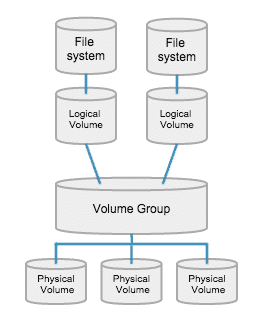
\includegraphics[width=0.65\textwidth]{lvm.png}
  \caption{Arquitectura LVM}
\end{figure}
\newpage
\subsubsection{Instalación de Ubuntu Server con RAID1}
\begin{enumerate}
  \item Descargamos la ISO desde \href{http://atcproyectos.ugr.es/esriie/ubuntu-16.04.5-server-amd64.iso}{aquí}.
  \item Creamos una máquina virtual con 1024MB RAM y dos discos duros VDI reservados dinámicamente de 10GB cada uno. Por último, montamos la ISO en el controlador IDE.
  \item  Arrancamos la máquina, marcamos idioma español y procedemos a la instalación.
  \item Elegimos España y la distribución de teclado Spanish/Spanish.
	\item Dejamos el nombre de la máquina en "ubuntu" y establecemos el nombre de usuario con nuestras iniciales. La clave será \textit{practicas,ISE}.
	\item No ciframos la carpeta personal, ya que usaremos FDE (\textit{Full Disk Encryption}).
	\item Aceptamos la zona horaria propuesta.
	\item Elegimos particionado manual.
	\item Damos Enter en ambos discos para crear las tablas de particiones.
	\item Comenzamos configurando RAID (\textit{Configurar RAID por software}).
	\item Creamos dispositivo MD (\textit{Multiple Devices}), elegimos RAID1, establecemos 2 discos en uso y 0 vacíos, los seleccionamos y damos a terminar.
	\item Pasamos a configurar LVM (\textit{Configurar el Gestor de Volúmenes Lógicos (LVM)}).
	\item Creamos el grupo de volúmenes, con nombre \textit{Servidor} y elegimos \textit{/dev/md0}.
	\item Creamos ahora los volúmenes lógicos sobre Servidor (\textit{swap} (1024MB),\textit{arranque} (200MB),\textit{hogar} (800MB) y \textit{raíz} (resto)). Por último, damos a terminar.
	\item Pasamos a la configuración del cifrado (\textit{Configurar los volúmenes cifrados}).
	\item Damos a \textit{Create encrypted volumes} y seleccionamos todos menos \textit{arranque} (si lo encriptamos no podremos arrancar el sistema).
	\item Mantenemos los parámetros predeterminados, por lo que elegimos \textit{Se ha terminado de definir la partición} en todos los casos.
	\item Damos \textit{Sí} a mantener la distribución existente, \textit{Finish} y establecemos la clave \textit{practicas,ISE} en todos los volúmenes.
	\item Por último, vamos a formatear los volúmenes y asignar los puntos de montaje. Para ello, elegimos las particiones (marcadas con el símbolo \textbf{\#}) \textit{arranque}, \textit{hogar} y \textit{raíz}. Seleccionamos \textit{Utilizar como: sistema de ficheros ext4 transaccional} y asignamos los puntos de montaje \textit{/boot}, \textit{/home} y \textit{/} respectivamente.
	\item Para la partición \textit{swap}, elegimos \textit{Utilizar como: área de intercambio}.
	\item Finalizamos el particionado y esperamos.
	\item Dejamos en blanco el campo de proxy y elegimos la opción \textit{Sin actualizaciones automáticas}, ya que queremos mantener el control total sobre el sistema.
	\item Dejamos seleccionado \textit{Standard system utilities} y pulsamos Enter.
	\item Instalamos en cargador de arranque en \textit{/dev/sda}.
	\item Una vez que el sistema esté instalado, iniciamos sesión y desbloqueamos los volúmenes cifrados.
	\item Pasamos ahora a instalar \textit{GRUB} en el otro disco. Para ello ejecutamos:
	\begin{lstlisting}
		$> sudo grub install /dev/sdb
	\end{lstlisting}

\end{enumerate}

\subsubsection{Configuración de red}

Necesitamos configurar la red de forma que las máquinas puedan comunicarse entre sí,con el \textit{host} y con el exterior. Para ello, seguiremos los siguientes pasos:
\begin{enumerate}
	\item Crear una red sólo-anfitrión.
	\begin{enumerate}
		\item En VirtualBox (¡no en la máquina!) damos a Archivo-Administrador de red anfitrión.
		\item Seleccionamos Crear y comprobamos que la IPv4a sea 192.168.56.1. En caso contrario, la modificamos.
		\item En la configuración de la máquina virtual Ubuntu, habilitamos el adaptador 2 (conectado a adaptador sólo-anfitrión)
	\end{enumerate}
	\item Añadir la interfaz y activarla.
	\begin{enumerate}
		\item Arrancamos la máquina.
		\item Editamos el archivo de interfaces mediante \textit{sudo nano /etc/network/interfaces}.
		\item Añadimos el siguiente código:
		\begin{lstlisting}
			# Host-only interface
			auto enp0s8
			iface enp0s8 inet static
			address 192.168.56.105
		\end{lstlisting}
		\item Salimos y guardamos.
		\item Activamos la interfaz con \textit{sudo ifup enp0s8}.
		\item Ejecutamos \textit{ip addr} y comprobamos que la interfaz tiene asignada la IP que configuramos (192.168.56.105).
	\end{enumerate}
	\item Comprobar que funciona.
		\begin{enumerate}
			\item Desde nuestro host, abrimos una terminal y ejecutamos \textit{ping 192.168.56.105 -c 5}. Deberíamos recibir las 5 respuestas.
			\item Desde la máquina virtual ejecutamos \textit{ping 192.168.56.1 -c 5}. Deberíamos recibir las 5 respuestas.
		\end{enumerate}
\end{enumerate}

\subsection{Sesión 2}
\subsubsection{Instalación de CentOS}
\begin{enumerate}
	\item Descargamos la ISO desde \href{http://atcproyectos.ugr.es/esriie/ubuntu-16.04.5-server-amd64.iso}{este enlace}.
	\item Creamos una máquina virtual con 1024MB de RAM y un disco duro de 10GB (elegimos la opción \textit{Fedora 64bits}). Por último, montamos la ISO.
	\item Seleccionamos \textit{Install CentOS Linux}.
	\item Elegimos Español (España).
	\item En \textit{Destino de la instalación} elegimos el único disco disponible y damos a \textit{Listo} y a \textit{Empezar instalación}.
	\item Creamos el usuario (iniciales como usuario y \textit{practicas,ISE} como clave). Establecemos también la contraseña del \textit{root} (\textit{practicas,ISE}).
\end{enumerate}

La temática de esta sesión es la siguiente: necesitamos espacio en \textit{/var} pero no tenemos suficiente. Para dar solución a ello, tendremos que seguir estos pasos:
\begin{enumerate}
	\item Añadir el disco a la máquina.
	\item Configurar el disco mediante \textit{LVM} y darle formato.
	\item Copiar los datos de \textit{/var} al nuevo volumen.
	\item Indicar al SO que monte el nuevo volumen en \textit{/var}.
	\item Borrar los datos antiguos de \textit{/var} (en la vida real ésto se haría un tiempo prudencial después para poder disponer de un backup.)
\end{enumerate}

Básicamente, tenemos que pasar del esquema actual:
\begin{figure}[H]
	\centering
	\begin{tikzpicture}[arrow/.style = {thick,-stealth}, node distance=2cm]
		\tikzset{set/.style={draw,rectangle,inner sep=0pt,align=center}}
		\node[fit={(0,0) (2,1)}, inner sep=0pt, draw=black, thick, text centered] (sda1) {sda1};
		\node[fit={(2,0) (4,1)}, inner sep=0pt, draw=black, thick, text centered] (sda2) {sda2};

		\node[fit={(2,2) (4,3)}, inner sep=0pt, draw=black, thick, text centered] (sda2pv) {sda2};

	\node[circle,above of=sda2pv, inner sep=0pt, draw=black, thick, text centered, minimum size = 1cm] (cl) {cl};

	\node[circle,above left of=cl, inner sep=0pt, draw=black, thick, text centered, minimum size = 1cm] (/) {/};

	\node[circle,above right of=cl, inner sep=0pt, draw=black, thick, text centered, minimum size = 1cm] (swap) {swap};


		\draw [decorate,decoration={brace,amplitude=10pt, raise=2.5pt, mirror}]	(6,0) -- (6,1) node [black,midway,xshift=1cm] {\footnotesize HDD};
		\draw [decorate,decoration={brace,amplitude=10pt, raise=2.5pt, mirror}]	(6,2) -- (6,3) node [black,midway,xshift=1cm] {\footnotesize PV};
		\draw [decorate,decoration={brace,amplitude=10pt, raise=2.5pt, mirror}]	(6,4) -- (6,5) node [black,midway,xshift=1cm] {\footnotesize VG};
		\draw [decorate,decoration={brace,amplitude=10pt, raise=2.5pt, mirror}]	(6,5.35) -- (6,6.35) node [black,midway,xshift=1cm] {\footnotesize LV};

		\draw [arrow] (sda2) -- (sda2pv);
		\draw [arrow] (sda2pv) -- (cl);
		\draw [arrow] (cl) -- (/);
		\draw [arrow] (cl) -- (swap);

	\end{tikzpicture}
\end{figure}

Al siguiente:
\begin{figure}[H]
	\centering
	\begin{tikzpicture}[arrow/.style = {thick,-stealth}, node distance=2cm]
		\tikzset{set/.style={draw,rectangle,inner sep=0pt,align=center}}
		\node[fit={(0,0) (2,1)}, inner sep=0pt, draw=black, thick, text centered] (sda1) {sda1};
		\node[fit={(2,0) (4,1)}, inner sep=0pt, draw=black, thick, text centered] (sda2) {sda2};

		\node[fit={(5,0) (7,1)}, inner sep=0pt, draw=black, thick, text centered] (sdb) {sdb};

		\node[fit={(2,2) (4,3)}, inner sep=0pt, draw=black, thick, text centered] (sda2pv) {sda2};
		\node[fit={(5,2) (7,3)}, inner sep=0pt, draw=black, thick, text centered] (sdbpv) {sdb};

	\node[circle,above of=sda2pv, inner sep=0pt, draw=black, thick, text centered, minimum size = 1cm] (cl) {cl};

	\node[circle,above left of=cl, inner sep=0pt, draw=black, thick, text centered, minimum size = 1cm] (/) {/};

	\node[circle,above of=cl, inner sep=0pt, draw=black, thick, text centered, minimum size = 1cm] (swap) {swap};

	\node[circle, above right of=cl, inner sep=0pt, draw=black, thick, text centered, minimum size = 1cm] (var) {/var};

		\draw [decorate,decoration={brace,amplitude=10pt, raise=2.5pt, mirror}]	(8,0) -- (8,1) node [black,midway,xshift=1cm] {\footnotesize HDD};
		\draw [decorate,decoration={brace,amplitude=10pt, raise=2.5pt, mirror}]	(8,2) -- (8,3) node [black,midway,xshift=1cm] {\footnotesize PV};
		\draw [decorate,decoration={brace,amplitude=10pt, raise=2.5pt, mirror}]	(8,4) -- (8,5) node [black,midway,xshift=1cm] {\footnotesize VG};
		\draw [decorate,decoration={brace,amplitude=10pt, raise=2.5pt, mirror}]	(8,5.35) -- (8,7) node [black,midway,xshift=1cm] {\footnotesize LV};

		\draw [arrow] (sda2) -- (sda2pv);
		\draw [arrow] (sdb) -- (sdbpv);
		\draw [arrow] (sda2pv) -- (cl);
		\draw [arrow] (sdbpv) -- (cl);
		\draw [arrow] (cl) -- (/);
		\draw [arrow] (cl) -- (swap);
		\draw [arrow] (cl) -- (var);

	\end{tikzpicture}
\end{figure}

\paragraph{Añadir el disco a la máquina}
Mediante el administrador de VirtualBox añadimos un nuevo disco (VDI, 10GB, reserva dinámica) a nuestra instancia.
\paragraph{Configurar el disco mediante \textit{LVM} y darle formato}
\begin{enumerate}
	\item Arrancamos la máquina.
	\item Comprobamos que el disco efectivamente ha sido detectado mediante \textit{lsblk}(\textbf{L}i\textbf{S}t \textbf{BL}oc\textbf{K} devices). Deberíamos ver el nuevo dispositivo \textit{/dev/sdb}. Podemos apreciar también aquí que \emph{CentOS} usa \textit{LVM} de forma nativa, bajo un grupo de volúmenes llamado \textit{cl}. También podemos ver como \textit{/boot} está sobredimensionado. Esto se hace para poder tener un backup del kernel antiguo en caso de que deba actualizarse.
	\item Como vamos a modificar elementos del sistema, nos logueamos como superusuario:
	\begin{lstlisting}
		$> su
	\end{lstlisting}
	\item Podemos ver los detalles de \textit{LVM} mediante los comandos \textit{lvdisplay} (\textit{\textbf{L}ogical \textbf{V}olume Display}), \textit{vgdisplay} (\textit{\textbf{V}olume \textbf{G}roup Display}) o \textit{pvdisplay} (\textit{\textbf{P}hysical \textbf{V}olume Display}).
	\item Creamos el volumen físico:
	\begin{lstlisting}
		#> pvcreate /dev/sdb
	\end{lstlisting}
	Podemos leer en el \textit{man} que podemos ejecutar el comando tanto en discos duros como en particiones. Comprobamos que se ha creado mediante \textit{pvdisplay}.
	\item Ahora debemos añadir el volumen físico al grupo de volúmenes existente (\textit{cl}). Para ello, ejecutamos
	\begin{lstlisting}
		#> vgextend cl /dev/sdb
	\end{lstlisting}
	Comprobamos que ha ido bien mediante \textit{vgdisplay}.
	\item Por último, debemos crear el volumen lógico. Para ello, ejecutamos el siguiente comando:
	\begin{lstlisting}
		#> lvcreate -L 5G -n newvar cl
	\end{lstlisting}
	Donde:
	\begin{itemize}
		\item -L indica el tamaño del volumen.
		\item -n indica el nombre del volumen.
	\end{itemize}
	Para finalizar, comprobamos que ha ido bien mediante \textit{lvdisplay}.
\end{enumerate}
En este momento \textit{LVM} ha sido configurado completamente.
\paragraph{Copiar los datos de \textit{/var} al nuevo volumen}
\begin{enumerate}
	\item Debemos comenzar creando un sistema de archivos en nuestro volumen lógico. Pero primero debemos ver cuál es el punto de montaje del mismo mediante \textit{lvdisplay} (campo \textit{LV Path}).
	\item Ahora ejecutamos el comando para crear el sistema de archivos:
	\begin{lstlisting}
		#> mkfs -t ext4 /dev/cl/newvar
	\end{lstlisting}
\end{enumerate}

\paragraph{Copiar los datos de \textit{/var} al nuevo volumen}
\begin{enumerate}
	\item Lo primero que debemos hacer es montar el volumen. Para ello ejecutamos
	\begin{lstlisting}
		#> mkdir /mnt/newvar
		#> mount /dev/cl/newvar /mnt/newvar
	\end{lstlisting}
	Comprobamos con \textit{mount}.
	\item Ahora debemos plantearnos lo siguiente: la copia debe realizarse de forma \emph{atómica}, es decir, nadie puede modificar ningún archivo, ya que esto generaría inconsistencias. Para ello, accedemos al modo de mantenimiento:
	\begin{lstlisting}
		#> systemctl isolate runlevel1.target
	\end{lstlisting}
	Introducimos de nuevo la clave del \textit{root}.
	\item Realizamos la copia de los ficheros:
	\begin{lstlisting}
		#> cp -a /var/. /mnt/newvar
	\end{lstlisting}
	Donde:
	\begin{itemize}
		\item -a indica que se deben copiar los archivos recursivamente, manteniendo enlaces y preservando el contexto. El contexto está compuesto por políticas de seguridad de \textit{SELinux} (\textit{\textbf{S}ecurity \textbf{E}nhanced Linux}) que controlan el acceso a recursos de los procesos.
		\item /var/. indica todos los archivos (incluidos los ocultos).
	\end{itemize}
	Comprobamos mediante \textit{ls -ahZ} sobre \textit{/var} y \textit{mnt/newvar}
\end{enumerate}

\paragraph{Indicarle al SO que monte el nuevo volumen en \textit{/var}}
\begin{enumerate}
	\item Abrimos el editor de texto sobre \textit{/etc/fstab}
	\begin{lstlisting}
		#> vi /etc/fstab
	\end{lstlisting}
	\item Pulsamos \textit{i} para acceder al modo de inserción y añadimos la siguiente línea:
	\begin{lstlisting}
		/dev/mapper/cl-newvar /var ext4 defaults 0 0
	\end{lstlisting}
	\item Salimos de vi (ESC, escribimos \textit{:wq} y Enter).
	\item Desmontamos el nuevo volumen:
	\begin{lstlisting}
		#> umount /mnt/newvar
	\end{lstlisting}
	\item Montamos los sistemas de archivos de \textit{/etc/fstab}:
	\begin{lstlisting}
		#> mount -a
	\end{lstlisting}
	Comprobamos ejecutando \textit{mount}.
\end{enumerate}

\paragraph{Borrar los datos antiguos de \textit{/var}}
Actualmente no tenemos acceso al antiguo \textit{/var} (el que tenemos montado actualmente es el nuevo).
\begin{enumerate}
	\item Comenzamos desmontando \textit{/var}:
	\begin{lstlisting}
		#> umount /dev/mapper/cl-newvar
	\end{lstlisting}
	\item Cambiamos el nombre de \textit{/var}:
	\begin{lstlisting}
		#> mv /var /var_old
	\end{lstlisting}
	\item Creamos \textit{/var} para que se pueda montar:
	\begin{lstlisting}
		#> mkdir /var
	\end{lstlisting}
	\item Restauramos el contexto de \textit{/var}:
	\begin{lstlisting}
		#> restorecon /var
	\end{lstlisting}
	\item Montamos la nueva partición \textit{/var}:
	\begin{lstlisting}
		#> mount -a
	\end{lstlisting}
	\item Salimos del modo de seguridad:
	\begin{lstlisting}
		#> systemctl isolate default
	\end{lstlisting}
	\item Eliminamos los archivos antiguos:
	\begin{lstlisting}
		#> rm -rf /var_old
	\end{lstlisting}
\end{enumerate}







\section{Preguntas de examen}
\subsection{Práctica 1}
\begin{enumerate}
  \item Si monto un RAID0 y un RAID1 con 2 HDD de 10GB, ¿cuánto espacio tengo disponible?
  \begin{solution}
    \begin{itemize}
      \item RAID0: 20GB, ya que no hay redundancia.
      \item RAID1: 10GB, ya que los datos se replican.
    \end{itemize}
  \end{solution}
  ¿Y si uso un HDD de 10GB y otro de 50GB?
  \begin{solution}
    \begin{itemize}
      \item RAID0: 60GB.
      \item RAID1: 10GB. Si tomáramos más espacio no podría replicarse.
    \end{itemize}
  \end{solution}
  \item Disponemos de un sistema con particiones \textit{home}, \textit{swap}, \textit{boot} y \textit{root}. Sólo podemos encriptar una de ellas. ¿Cuál elegirías?
  \begin{solution}
    SWAP, ya que contiene datos de la RAM, como claves, archivos de las aplicaciones, etc.
  \end{solution}
	\item ¿Qué diferencias hay entre \textit{EXT2} y \textit{EXT4}?
	\begin{solution}
		\textit{EXT4}, a diferencia de \textit{EXT2}, admite \textit{journaling}, es decir, un diario que permite restablecer los datos anteriores a una transacción en caso de que ésta falle. Esta técnica permite al sistema de archivos volver a un estado coherente si se produce un corte de electricidad o cualquier otro fallo durante una transacción. Otra característica muy interesante de \textit{EXT4} es el asignamiento multi-bloque, que permite asignar varios bloques en una misma llamada.
	\end{solution}
	\item ¿Qué diferencias hay entre:
	\begin{itemize}
		\item \textit{cp -a /var /newvar}
		\item \textit{cp -a /var/ /newvar}
		\item \textit{cp -a /var/* /newvar}
		\item \textit{cp -a /var/. /newvar}
	\end{itemize}
	?
	\begin{solution}
		\begin{itemize}
			\item \textit{cp -a /var /newvar} copia la carpeta, no el contenido. Es decir, quedaría \textit{/newvar/var/archivos}
			\item \textit{cp -a /var/* /newvar} no copia los archivos ocultos.
			\item \textit{cp -a /var/. /newvar} copia todos los archivos (visibles y ocultos) y además mantiene el contexto.
		\end{itemize}
	\end{solution}
\end{enumerate}




\end{document}
